\chapter{Background}
\section{Scenario}
Nell'ambiente in cui viviamo siamo circondati da sempre più entità
computazionali eterogenee tra loro. Device come smartphone, wearable, display
pubblici, droni, insegne digitali, sensori di ogni tipo, stanno sempre più
pervadendo il nostro ambiente quotidiano. L'interazione tra questi dispositivi
vicini gioca un ruolo fondamentale in settori emergenti come Internet-of-Things,
Smart City, reti di sensori o più in generale in sistemi collettivi
adattivi. Quando si parla di questo tipo di sistemi si deve tenere in
considerazione l'elevato numero di dispositivi diversi di cui essi sono
composti, quindi il numero di piattaforme, tecnologie, modelli di
programmazione, protocolli, etc.. Le specifiche di basso livello, come
efficienza, organizzazione e coordinazione di questi dispositivi in un sistema
distribuito, influenzano pesantemente le scelte di design di quest'ultimo. Ne
risulta un sistema rigido, costoso da mantenere, estendere ed eventualmente
scalare.

Sorge quindi la necessità di un modello di programmazione più ad alto livello,
che consenta di astrarre i dettagli di sistema in larga scala, delegando allo
strato sottostante tutte le questioni legate al \textit{deployment}, che possa
occuparsi di tutti i requisiti non funzionali come le proprietà di
auto-organizzazione e auto-adattività. Possono essere elencate tre
caratteristiche chiave\cite{DBLP:journals/computer/BealPV15} che questo strato dovrebbe semplificare:
\begin{itemize}
\item i meccanismi di coordinazione dovrebbero essere nascosti e i gli
  sviluppatori non dovrebbero essere tenuti a interagire con essi;
\item la composizione di moduli o sottosistemi dovrebbe essere semplice e
  trasparente;
\item sottosistemi distinti necessitano di meccanismi di coordinazione per distinti
regioni e tempo.
\end{itemize}


\section{Aggregate computing}
L'osservazione che viene fatta spesso è che spesso il comportamento collettivo
di un sistema interessa più del singolo dispositivo di cui è composto, ma i
linguaggi di programmazione classici, orientati al singolo dispositivo, forzano
lo sviluppatore a porre l'attenzione sui singoli device e all'interazione tra di
essi.

Il paradigma di \textit{aggregate computing} si propone di risolvere le
precedenti questioni tramite i seguenti principi:
\begin{enumerate}
\item il dispositivo programmato è una regione dell'ambiente computazionale e
  prescinde dagli specifici dettagli;
\item il programma è specificato come manipolazione di strutture dati con
  estensione temporale e spaziale attraverso quella regione;
\item queste manipolazioni sono effettivamente eseguite dai singoli dispositivi
  nella regione, usando meccanismi di coordinazione resilienti e interazioni
  basate sulla prossimità. \cite{DBLP:journals/computer/BealPV15}
\end{enumerate}

Un esempio di utilizzo nel mondo reale potrebbe essere un servizio che,
utilizzando interazioni tra gli smartphone per stimare la densità di popolazione
presente in un area o ad un certo evento, possa fornire indicazioni relative a
zone che possono essere considerate pericolose perché troppo dense, che percorso
seguire eventualmente per disperderle; più in generale possono essere erogate
indicazioni per raggiungere un punto scelto evitando le zone più pericolose.

% continuum-like (traduzione?)
% TODO: figura 2
% http://openmap.bbn.com/~jbeal/Publications/Computer-AggregateProgramming-Preprint-2015.pdf
La figura 2a mostra come con un linguaggio di programmazione orientato al
singolo device il programmatore sia costretto a porre la propria attenzione
sull'interazione tra i dispositivi, mentre si occupa di modellare localmente un
comportamento che dovrà produrre un certo effetto globale.
Invece, con l'utilizzo della programmazione aggregata (figura 2b), si è liberi
di pensare in maniera più naturale tramite strutture dati
\textit{continuum-like} e servizi che possono essere composti in maniera modulare.
Nello specifico il servizio di \textit{crowd estimation} produce in output una
struttura dati distribuita --- un campo computazionale --- che associa ad ogni
posizione una densità di popolazione. Questo è l'input dei servizi che poi si
vogliono costruire: navigazione, segnalazione delle zone di pericolo ed
istruzioni per un'eventuale evacuazione.

La capacità di separare la logica dei servizi dall'implementazione della
comunicazione e dai protocolli utilizzati per questa, orientano verso lo
sviluppo di applicazioni distribuite più complesse, ma allo stesso tempo
modulari, riusabili e facilmente estendibili.

L'obiettivo della programmazione aggregata è nascondere la complessità di
coordinare un sistema distribuito utilizzando diversi livelli di astrazione.
Nel tempo sono stati sviluppati diversi modelli di programmazione aggregata, ma
la maggior parte di questi sono troppo specializzati per singole istanze di
problemi e non sufficientemente generici da risolvere intere classi di
problemi\cite{beal2012}.

Tra questi però è stati sviluppato il \textit{field calculus}: un insieme di
costrutti fondamentali, derivati dagli elementi comuni degli altri metodi e che
modellano la computazione e l'interazione tra un largo numero di dispositivi
sparsi nello spazio.

% TODO figura 1
% https://ieeexplore.ieee.org/stamp/stamp.jsp?tp=&arnumber=8064162
\subsection{Field calculus}
Utilizzando diversi approcci di programmazione aggregata emergono certi pattern
che si ripetono. Il \textit{field calculus} \cite{Viroli2013} cattura queste
caratteristiche in un minuscolo linguaggio universale adatto all'analisi
matematica.

L'elemento fondamentale del \textit{field calculus} è il campo computazionale,
ispirato a concetti fisici come i campi magnetici, che associa ad ogni
dispositivo in rete un valore locale. Ogni valore, funzione o variabile è un
campo: per esempio una collezione di sensori di temperatura produce un campo di
temperature dell'ambiente, una collazione di accelerometri di smartphone produce
un campo di direzioni, una notifica di un'applicazione produce un campo di
messaggi.

I campi sono generati e manipolati utilizzando quattro costrutti fondamentali:
\begin{itemize}
\item \textbf{Funzioni}: \texttt{b($e_1,\ldots, e_n$)} applica la funzione \texttt{b}
  agli argomenti \texttt{$e_1,\ldots, e_n$}. Queste sono funzioni matematiche,
  logiche o algoritmiche stateless, oppure sensori, attuatori, funzioni definite
  dall'utente o importate.

\item \textbf{Dynamics}: \texttt{rep(x<-v) \{$s_1;\ldots;s_n$\}} definisce una variabile
  locale di stato \texttt{x} inizializzata con il valore \textit{v} e aggiornata
  periodicamente con il risultato dell'esecuzione gli statement
  \texttt{{$s_1;\ldots;s_n$}} che compongono il suo corpo. In questo modo viene
  definito un campo che cambia nel tempo.

\item \textbf{Iterazioni}: \texttt{nbr($s$)} acquisisce un campo che associa ad ogni
  device tra tutti i dispositivi vicini (incluso se stesso), il loro ultimo
  valore di \texttt{$s$}. Questo campo può essere poi processato da funzioni
  built-in chiamate \textit{hood}, che permettono di ridurre il campo ad un
  valore, per esempio il minimo.

\item \textbf{Restrizione}: \texttt{if($e$) \{$s_1;\ldots;s_n$\} else
    \{$s'_1;\ldots;s'_m$\}} partiziona la rete in due regioni disgiunte: dove la
  \texttt{$e$} è vero viene eseguito \texttt{$s_1;\ldots;s_n$}, nell'altra parte,
  invece, è eseguito \texttt{$s'_1;\ldots;s'_n$}. È importante menzionare il
  fatto che le due diramazioni sono incapsulate e non possono avere effetti al
  di fuori del loro sottospazio.
\end{itemize}

Questi costrutti permettono la portabilità, indipendenza dall'infrastruttura e
interazione con servizi non aggregati.

\subsection{Building blocks}
Il successivo livello di astrazione serve ad aggiungere resilienza. È
identificata una collezione di operatori ``building block'' generici finalizzata
a una coordinazione robusta delle applicazioni. I meccanismi di questo livello
(quello in mezzo nella Figura 3), sono \textit{auto-stabilizzati}, cioé si
adattano ai cambiamenti della rete o dei dati in input, scalabili a reti di
grandi dimensioni e preservano la caratteristica di resilienza quando sono
composti tra di loro\cite{7056345}.

La collezione è composta da tre operatori di coordinazione generali e
dall'operatore built-in \texttt{if}. I tre operatori sono:
\begin{itemize}
\item \textbf{G}: che distribuisce un informazione nello spazio. Questo
  operatore generalizza operazioni molto comuni come la stima della distanza e
  messaggi broadcast.
\item \textbf{C}: che aggrega un informazione in uno o più nodi.
\item \textbf{T}: che generalizza un timer il cui rateo di aggiornamento può
  variare nel tempo.
\end{itemize}

\subsection{General-purpose API}
È un ulteriore livello di astrazione (il secondo dall'alto nella Figura 3) che
mira a soddisfare la necessità più generiche fornendo delle API di alto livello:
funzioni come \texttt{distanceTo()} o \texttt{broadcast()}. Queste sono
implementate a partire dai costrutti, già descritti, di cui è formato il livello
sottostante e consentono di scrivere programmi più facilmente.

Queste API possono essere usate e composte tra loro per scrivere applicazioni
distribuite senza proccuparsi di meccanismi di coordinazione. Infatti costruire
delle API utilizzando degli operatori \textit{resilient} assicura che i servizi
lo siano a loro volta.

% TODO: La sintassi?
\section{Protelis}
Il \textit{field calculus} è un fondamento teoretico importante, ma troppo di
basso livello se paragonato all'ecosistema costruito intorno ai linguaggi di
programmazione moderni. L'assenza di tool, librerie e la mancata integrazione
con piattaforme esistenti lo rendono uno strumento efficace, ma
isolato. Protelis si pone come obiettivo quello di integrare un interprete di
\textit{field calculus} in un architettura reale, ovvero che si interfacci con
hardware, operativo e piattaforme esistenti. È importante che questa
implementazione sia facilmente portabile sia su un ambiente simulato che su una
rete di dispositivi reale.

La sintassi del linguaggio è di facile apprendimento in quanto si ispira a
quella dei linguaggi C-like come Java.

\subsection{Protelis nel mondo scientifico}
Esistono situazioni reali nelle quali l'accesso a servizi basati sul cloud non è
possibile e le infrastrutture di rete presenti in una determinata area non sono
adatte ad un'elevata presenza di dispositivi, ne consegue che qualsiasi tipo di
tentativo di coordinare due o più dispositivi, passando per un aggregatore di
informazioni, è soggetto alla congestione della rete, risultando di scarsa
efficacia o addirittura inutilizzabile. È il caso, per esempio, delle riunioni
di massa: grandi eventi pubblici a cui partecipano un numero ingente di persone.
Per risolvere problemi legati a questo tipo di situazioni è necessario
utilizzare un approccio distribuito, che possa basare il proprio funzionamento
sull'interazione dei singoli nodi che fanno parte di una rete, senza affidarsi a
un sistema di coordinazione centralizzata.

Protelis ha una potenza espressiva molto elevata: è in grado di esprimere
algoritmi distribuiti complessi in poche righe di codice. È infatti stato
sfruttato per implementare diversi algoritmi distribuiti. Tra questi i più
rilevanti sono: \textit{rendezvous} ad una riunione di
massa\footnote{https://protelis.github.io/peer-to-peer-route-planning}
\cite{Protelis}, algoritmo che consente a due persone che partecipano ad un
evento di massa di incontrarsi in un punto intermedio, evitando zone di alta
densità; stima di pericolosità di una zona per sovrappopolazione e notifica di
pericolo\footnote{https://protelis.github.io/crowd-warning} \cite{7056345}, che
consente di stimare la pericolosità di una zona, basandosi sulla densità di
dispositivi presenti in essa, e come disperdere l'eventuale massa di persone in
maniera efficiente.

Un altro ipotetico ambito di utilzzo è la gestione dei servizi in una
rete\footnote{https://protelis.github.io/network-management} \cite{Protelis}: i
servizi di rete sono spesso \textit{legacy} e spesso non riescono a gestire un
errore degli altri servizi da cui dipendono. Quindi potrebbero continuare a
comportarsi in maniera non definita, modificando in maniera inconsistente il
proprio stato. Reagire in maniera coerente ad un errore del genere richiede un
sistema di coordinazione tra i servizi coinvolti per riavviare l'intero
stack. La programmazione aggregata risolve questo problema tramite i propri
meccanismi di sincronizzazione nativi.

\subsection{Architettura di Protelis}\label{subsec:Architettura di Protelis}
\begin{figure}
  \subfloat[Funzionamento di Protelis]{
    % 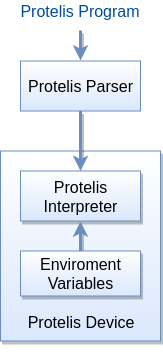
\includegraphics[height=5.5cm]{media/protelis-architecture.png}
    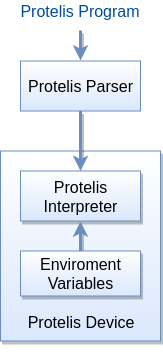
\includegraphics[height=6.2cm]{media/protelis-architecture.png} \label{fig:architettura-protelis}
  }\hfill
  \subfloat[Estendibilità di Protelis]{
    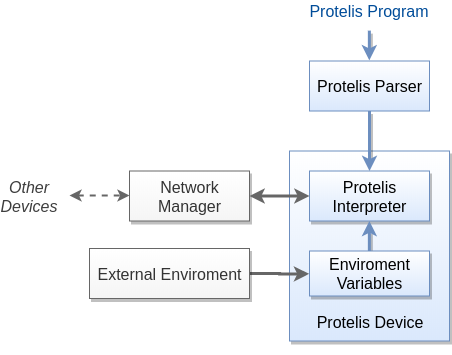
\includegraphics[height=6.2cm]{media/extend-protelis.png}
    \label{fig:estensione-protelis}
  }
  \caption{Architettura astratta di Protelis (a) e meccanismo di estendibilità
    previsto dal linguaggio (b).}
\end{figure}

Protelis è un linguaggio di programmazione aggregato, fortemente influenzato da
Proto\cite{Proto}, che risolve questi problemi utilizzando una macchina
virtuale\cite{Protelis}.  Inizialmente un parser traduce un programma Protelis
in una rappresentazione comprensibile all'interprete, che può eseguirlo, in
seguito, a intervalli regolari. L'interprete può interagire con l'ambiente
circostante, implementato tramite tuple \textit{(chiave, valore)} (Figura
\ref{fig:architettura-protelis}).

La duplice possibilità di poter eseguire un interprete Protelis in due contesti
diversi, quali sono un ambiente simulato e quello reale, evidenziano la
necessità dell'introduzione di un componente middleware, che gestisca la
comunicazione tra le macchine virtuali in maniera completamente trasparente a
queste ultime (Figura \ref{fig:estensione-protelis}). Sfruttando la
caratteristica del polimorfismo dei linguaggi ad oggetti, questo modello può
essere facilmente specializzato in entrambi i contesti precedentemente citati.

La piattaforma di supporto scelta per l'implementazione è Java, scelta
supportata da molteplici motivi\cite{Protelis}. I principali sono: la sua
portabilità, il meccanismo interno della reflection che esso supporta e il
sempre crescente numero di dispositivi embedded a basso costo che supportano
Java. Un altro fattore determinante è l'efficienza in termini di costo di
risorse che le implementazioni Java hanno raggiunto, rendendolo competitivo con
linguaggi di basso livello come il C o C++.

La scelta del linguaggio Java come piattaforma di supporto permette a Protelis
di essere interoperabile con esso, di conseguenza può essere integrato con un
vastissimo numero di API \textit{domain-specific} il cui ecosistema è dotato.
